\documentclass{beamer}

\mode<presentation>
\usepackage{amsmath}
\usepackage{amssymb}
%\usepackage{advdate}
\usepackage{adjustbox}
%\usepackage{subcaption}
\usepackage{enumitem}
\usepackage{multicol}
\usepackage{mathtools}
\usepackage{listings}
\usepackage{url}
\usetheme{Boadilla}
\usecolortheme{lily}
\setbeamertemplate{footline}
{
  \leavevmode%
  \hbox{%
  \begin{beamercolorbox}[wd=\paperwidth,ht=2.25ex,dp=1ex,right]{author in head/foot}%
    \insertframenumber{} / \inserttotalframenumber\hspace*{2ex} 
  \end{beamercolorbox}}%
  \vskip0pt%
}
\setbeamertemplate{navigation symbols}{}
\providecommand{\nCr}[2]{\,^{#1}C_{#2}} % nCr
\providecommand{\nPr}[2]{\,^{#1}P_{#2}} % nPr
\providecommand{\mbf}{\mathbf}
\providecommand{\pr}[1]{\ensuremath{\Pr\left(#1\right)}}
\providecommand{\qfunc}[1]{\ensuremath{Q\left(#1\right)}}
\providecommand{\sbrak}[1]{\ensuremath{{}\left[#1\right]}}
\providecommand{\lsbrak}[1]{\ensuremath{{}\left[#1\right.}}
\providecommand{\rsbrak}[1]{\ensuremath{{}\left.#1\right]}}
\providecommand{\brak}[1]{\ensuremath{\left(#1\right)}}
\providecommand{\lbrak}[1]{\ensuremath{\left(#1\right.}}
\providecommand{\rbrak}[1]{\ensuremath{\left.#1\right)}}
\providecommand{\cbrak}[1]{\ensuremath{\left\{#1\right\}}}
\providecommand{\lcbrak}[1]{\ensuremath{\left\{#1\right.}}
\providecommand{\rcbrak}[1]{\ensuremath{\left.#1\right\}}}
\theoremstyle{remark}
\newtheorem{rem}{Remark}
\newcommand{\sgn}{\mathop{\mathrm{sgn}}}

\providecommand{\res}[1]{\Res\displaylimits_{#1}} 
\providecommand{\norm}[1]{\lVert#1\rVert}
\providecommand{\mtx}[1]{\mathbf{#1}}

\providecommand{\fourier}{\overset{\mathcal{F}}{ \rightleftharpoons}}
%\providecommand{\hilbert}{\overset{\mathcal{H}}{ \rightleftharpoons}}
\providecommand{\system}{\overset{\mathcal{H}}{ \longleftrightarrow}}
	%\newcommand{\solution}[2]{\textbf{Solution:}{#1}}
%\newcommand{\solution}{\noindent \textbf{Solution: }}
\providecommand{\dec}[2]{\ensuremath{\overset{#1}{\underset{#2}{\gtrless}}}}
\newcommand{\myvec}[1]{\ensuremath{\begin{pmatrix}#1\end{pmatrix}}}

\title{Matrices in Geometry - 1.5.25}
\author{EE25BTECH11037  Divyansh}
\date{Aug, 2025}

\begin{document}

\maketitle

%\section*{Outline}
\begin{frame}
\tableofcontents
\end{frame}
\section{Problem}
\begin{frame}
\frametitle{Problem Statement}
In what ratio does the point \myvec{\frac{24}{11} \\ y} divide the line segment joining the points \textbf{P}=\myvec{2 \\ -2} and \textbf{Q}=\myvec{3 \\ 7}? Also find the value of y.

\end{frame}

\section{Solution}
\begin{frame}{Solution}
   $P\myvec{2\\-2}$, $Q\myvec{3\\7}$ and a point $R  \myvec{\frac{24}{11} \\ y}$ on $PQ$. \\
   Let $R$ divide $PQ$ internally in the ratio $\lambda:1$.\\

   \begin{enumerate}[label=\alph*)]
       \item By section formula,
       \begin{align*}
            \myvec{\frac{24}{11} \\ y}= \dfrac{\myvec{2 \\ -2} + \lambda\myvec{3 \\ 7}}{1+\lambda}
        \end{align*}
        \item Cross-multilying
        \begin{align*}
            \myvec{\brak{\lambda+1}\frac{24}{11} \\ \brak{\lambda+1}y}= \myvec{2+3\lambda \\ -2+7\lambda}
        \end{align*}
   \end{enumerate}
\end{frame}



\begin{frame}{Solution}
\begin{enumerate}[start=3,label=\alph*)]
    \item Solving for $\lambda$ and cross-multiplying, we get 
    \begin{align*}
        24\lambda + 24 = 22 + 33\lambda \implies 9\lambda=2 \implies \lambda=\frac{2}{9}
    \end{align*}

    \item Substituting the value of $\lambda$ above, we get 
    \begin{align*}
        y\brak{\frac{2}{9} +1}=-2+7\times\frac{2}{9} \implies 11y =-18+14 \implies y=\frac{-4}{11}
    \end{align*}
\end{enumerate}
\end{frame}

\section{Final Answer}
\begin{frame}{Final Answer}
    Hence, the final answer is $\fbox{\lambda = \dfrac{2}{9}} \; \text{and} \; \fbox{y = \dfrac{-4}{11}}$

\begin{figure}[H]
    \centering
    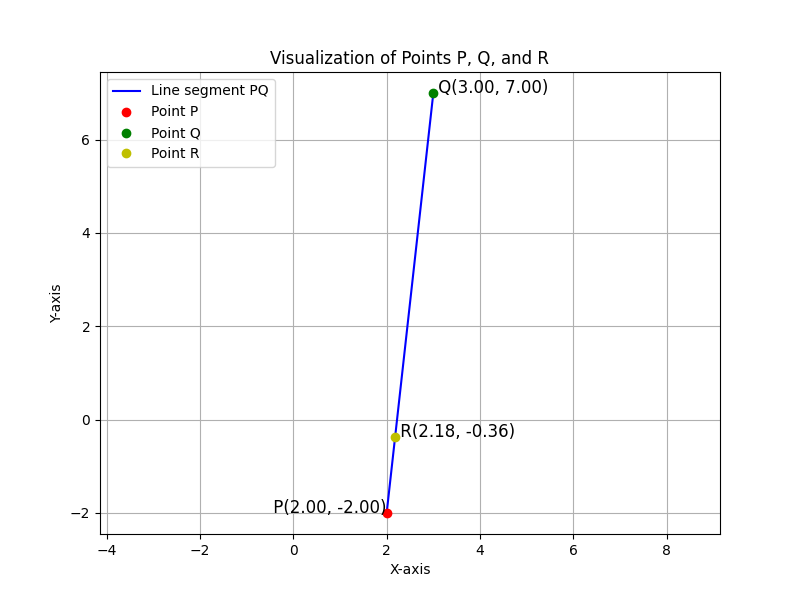
\includegraphics[width=0.5\columnwidth]{figs/1.png}
    \caption{Plot for 1.5.25}
    \label{fig:placeholder}
\end{figure}
\end{frame}


\end{document}

